\documentclass{standalone}
\usepackage{tikz}
\begin{document}%
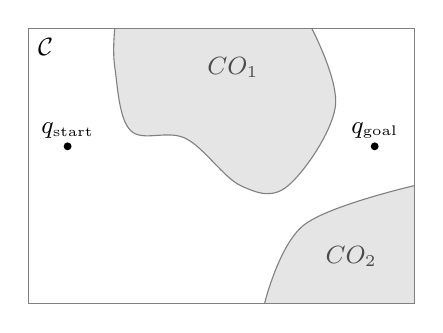
\begin{tikzpicture}[font=\small]

\ifdefined\argstart
\fi

\ifdefined\argcandidatesa
   \def\drawcandidatesa{}
\fi

\ifdefined\argcandidatea
   \def\drawcandidatea{}
   \def\drawcandidatesa{}
\fi

\ifdefined\argcandidateaevaled
   \def\drawcandidatea{}
   \def\drawcandidateaevaled{}
\fi

\ifdefined\argcandidatesb
   \def\drawcandidateaevaled{}
   \def\drawcandidatesb{}
\fi

\ifdefined\argcandidateb
   \def\drawcandidateaevaled{}
   \def\drawcandidateb{}
   \def\drawcandidatesb{}
\fi

\ifdefined\argcandidatebevaled
   \def\drawcandidateaevaled{}
   \def\drawcandidateb{}
   \def\drawcandidatebevaled{}
\fi

\ifdefined\argcandidatesfinal
   \def\drawcandidateaevaled{}
   \def\drawcandidatebevaled{}
   \def\drawcandidatefinalevaled{}
   \def\drawcandidatesb{} % same candidates
\fi

\ifdefined\argcandidatefinal
   \def\drawcandidateaevaled{}
   \def\drawcandidatebevaled{}
   \def\drawcandidatefinal{}
   \def\drawcandidatefinalevaled{}
   \def\drawcandidatesb{} % same candidates
\fi

% obstacle 1 fill
\fill[black!10] plot [smooth,tension=0.6] coordinates {
   (3.6,3.5) (3.9,2.5) (3.3,1.5) (2.7,1.5)
   (2.0,2.1) (1.3,2.2) (1.1,3.0) (1.1,3.5)};

% obstacle 2 fill
\fill[black!10] plot [smooth,tension=0.6] coordinates {
   (3.0,0.0) (3.5,1.0) (4.9,1.5)};
\fill[black!10] (4.9,1.5) -- (4.9,0.0) -- (3.0,0.0) -- cycle;

% obstacle 1 boundary
\draw[black!50] plot [smooth,tension=0.6] coordinates {
   (3.6,3.5) (3.9,2.5) (3.3,1.5) (2.7,1.5)
   (2.0,2.1) (1.3,2.2) (1.1,3.0) (1.1,3.5)};

% obstacle 2 boundary
\draw[black!50] plot [smooth,tension=0.6] coordinates {
   (3.0,0.0) (3.5,1.0) (4.9,1.5)};

% obstacle labels
\node[text=black!70] at (2.6,3.0) {$CO_1$};
\node[text=black!70] at (4.1,0.6) {$CO_2$};

% path
%\draw plot [smooth,tension=0.6,thick] coordinates {
%   (0.5,2.0) (1.0,1.0) (2.8,1.0) (4.0,1.9) (4.4,2.2)};

% first candidate paths
%\draw[thick,densely dashed] plot [smooth,tension=0.6] coordinates {
%   (0.5,2.0) (1.0,1.0) (2.8,1.0) (4.0,1.9) (4.4,2.2)};

\ifdefined\drawcandidatea
   \draw[line width=0.3cm,line cap=round,black!50,opacity=0.6] plot [smooth,tension=0.6] coordinates {
      (0.5,2.0) (2.45,1.9) (4.4,2.0)};
\fi

\ifdefined\drawcandidateb
   \begin{scope}
      \clip (0,0) rectangle (2.0,3.5);
      \draw[line width=0.3cm,line cap=round,black!50,opacity=0.6] plot [smooth,tension=0.6] coordinates {
         (0.5,2.0) (2.45,1.9) (4.4,2.0)};
   \end{scope}
   \begin{scope}
      \clip (2.0,0) rectangle (4.9,3.5);
      \draw[line width=0.3cm,line cap=round,black!50,opacity=0.6] plot [smooth,tension=0.6] coordinates {
         (2.0,1.91) (2.8,2.3) (4.4,2.0)};
   \end{scope}
\fi

\ifdefined\drawcandidatefinal
   \begin{scope}
      \clip (0,0) rectangle (2.0,3.5);
      \draw[line width=0.3cm,line cap=round,black!50,opacity=0.6] plot [smooth,tension=0.6] coordinates {
         (0.5,2.0) (2.45,1.9) (4.4,2.0)};
   \end{scope}
   \begin{scope}
      \clip (2.0,0) rectangle (4.9,3.5);
      \draw[line width=0.3cm,line cap=round,black!50,opacity=0.6] plot [smooth,tension=0.6] coordinates {
         (2.0,1.91) (2.9,1.2) (4.4,2.0)};
   \end{scope}
\fi

\ifdefined\drawcandidatesa
   \draw[thick,densely dashed] plot [smooth,tension=0.6] coordinates {
      (0.5,2.0) (2.45,1.9) (4.4,2.0)};

   \draw[thick,densely dashed] plot [smooth,tension=0.6] coordinates {
      (0.5,2.0) (2.45,2.5) (4.4,2.0)};

   \draw[thick,densely dashed] plot [smooth,tension=0.6] coordinates {
      (0.5,2.0) (2.45,0.8) (4.4,2.0)};
\fi

\ifdefined\drawcandidatesb
   \draw[thick,densely dashed] plot [smooth,tension=0.6] coordinates {
      (0.5,2.0) (2.45,1.9) (4.4,2.0)};

   \draw[thick,densely dashed] plot [smooth,tension=0.6] coordinates {
      (0.5,2.0) (2.45,2.5) (4.4,2.0)};

   \draw[thick,densely dashed] plot [smooth,tension=0.6] coordinates {
      (0.5,2.0) (2.45,0.8) (4.4,2.0)};

   \draw[thick,densely dashed] plot [smooth,tension=0.6] coordinates {
      (2.0,1.91) (2.8,2.3) (4.4,2.0)};

   \draw[thick,densely dashed] plot [smooth,tension=0.6] coordinates {
      (2.0,1.91) (2.9,1.2) (4.4,2.0)};
\fi

\ifdefined\drawcandidateaevaled
   \begin{scope}
      \clip (1.5,0) rectangle (2.24,3.5);
      \draw[ultra thick] plot [smooth,tension=0.6] coordinates {
         (0.5,2.0) (2.45,1.9) (4.4,2.0)};
   \end{scope}
   \begin{scope}
      \clip (2.24,0) rectangle (2.5,3.5);
      \draw[ultra thick,red] plot [smooth,tension=0.6] coordinates {
         (0.5,2.0) (2.45,1.9) (4.4,2.0)};
   \end{scope}
\fi

\ifdefined\drawcandidatebevaled
   \begin{scope}
      \clip (2.8,0) rectangle (3.78,3.5);
      \draw[ultra thick,red] plot [smooth,tension=0.6] coordinates {
         (2.0,1.91) (2.8,2.3) (4.4,2.0)};
   \end{scope}
   \begin{scope}
      \clip (3.78,0) rectangle (4.9,3.5);
      \draw[ultra thick] plot [smooth,tension=0.6] coordinates {
         (2.0,1.91) (2.8,2.3) (4.4,2.0)};
   \end{scope}
\fi

\ifdefined\drawcandidatefinalevaled
   \begin{scope}
      \clip (0,0) rectangle (2.24,3.5);
      \draw[ultra thick] plot [smooth,tension=0.6] coordinates {
         (0.5,2.0) (2.45,1.9) (4.4,2.0)};
   \end{scope}
   \draw[ultra thick] plot [smooth,tension=0.6] coordinates {
      (2.0,1.91) (2.9,1.2) (4.4,2.0)};
\fi

% path endpoints / labels
\fill[black] (0.5,2.0) circle (0.05cm);
\fill[black] (4.4,2.0) circle (0.05cm);
\node at (0.5,2.2) {$q_{\mbox{\tiny start}}$};
\node at (4.4,2.2) {$q_{\mbox{\tiny goal}}$};

% C label
\node[text=black,anchor=north west] at (0.0,3.5) {$\mathcal{C}$};

% C-space border
\draw[black!50] (0,0) rectangle (4.9,3.5);

% add a grid at 1cm resolution
%\draw[step=1cm,gray,very thin] (0,0) grid (5,4);

\end{tikzpicture}%
\end{document}
